\documentclass[12pt]{article}
\usepackage[utf8]{inputenc}
\usepackage[ngerman]{babel}
\usepackage[T1]{fontenc}
\usepackage{amsmath}
\usepackage{amssymb}
\usepackage{xcolor}
\usepackage{scrlayer-scrpage}
\pagestyle{scrheadings}
\usepackage{endnotes}
\usepackage{siunitx}
\usepackage{makeidx}
\usepackage{graphicx}
\usepackage{float}
\usepackage{mdframed}
\usepackage[useregional]{datetime2}
\makeindex
\usepackage{hyperref}
\let\footnote=\endnote
\parindent0pt
\sloppy	

\renewcommand{\notesname}{\vspace*{-1.2cm}}

\renewcommand{\theenumi}{(\roman{enumi})}
\renewcommand{\labelenumi}{\theenumi}
\renewcommand\labelitemi{{\boldmath$\cdot$}}
\renewcommand{\d}{\operatorname{d}}
\renewcommand{\i}{\operatorname{i}}
\newcommand{\abs}[1]{\ensuremath{\left\vert#1\right\vert}}
\newcommand{\dabs}[1]{\ensuremath{\left\Vert#1\right\Vert}}
\newcommand{\skalar}[1]{\ensuremath{\left\langle#1\right\rangle}}
\renewcommand{\det}{\operatorname{det}}

\newcommand\tab[1][1cm]{\hspace*{#1}}

\newenvironment{Code}{\begin{mdframed}[topline=false,bottomline=false,linewidth=1pt]\begin{scriptsize}\begin{tt}}
{\end{tt}\end{scriptsize}\end{mdframed}}
\newenvironment{Kasten}{\begin{mdframed}[linewidth=1pt]}{\end{mdframed}}
\newenvironment{Beweis}{\begin{mdframed}[topline=false,bottomline=false,linewidth=1pt]\begin{scriptsize}}
{\end{scriptsize}\end{mdframed}}
\newenvironment{Fig}{\begin{figure}[H]
\begin{center}}{\end{center}\end{figure}}

\setcounter{section}{-1}

\begin{document}
%\begin{folding}{Titel}
\chead{}
\ihead{}
\ohead{}
\begin{center}
\title{Ebene Kurven}
\author{-}
\date{30.11.2022}

\vspace*{3cm}
\rule{\linewidth}{1pt}\\
\vspace{0.5cm}
\LARGE \textbf{Computerpraktikum}\\
\large Ebene Kurven\\
\vspace{0.5cm}
\rule{\linewidth}{1pt}\\
\vspace{0.5cm}\large Bei -\\
\vspace{4cm}
\large\textbf{Von -}\\
\normalsize Mit -\\
\vfill
\scriptsize Wintersemester 2022/2023\\
30.11.2022
\end{center}
\newpage
\chead{Ebene Kurven}
\ihead{30.11.2022}
\ohead{}
\tableofcontents
\newpage
\setcounter{page}{1}
\cfoot{\pagemark}
%\end{folding}
\section{Vorwort}
Dieser Teil ist eine Ansammlung von mehr oder weniger unzusammenhängenden Anmerkungen und Gedanken zu dem Projekt und kann bis auf den folgenden Teil 0.1 Notation übersprungen werden.\\

Mein Partner Manuel Müller und ich haben uns mit Projekt 1 \glqq Ebene Kurven und Kurvenscharen\grqq{}\footnote{Jetzt im Nachhinein fällt mir auf, dass wir das Thema Kurvenscharen scheinbar etwas zu kurz behandelt haben.} beschäftigt.\\

Für das Projekt wurde \textit{Maple 2022} verwendet. Ich weiß leider nicht, wie es mit der Rückwärtskompatibilität aussieht. Falls Sie Probleme mit einem der Skripte haben, können Sie sich gerne an mich wenden, ansonsten liegen diesem Dokument einige \textit{Maple}-Worksheets bei, welche sich mit den einzelnen Teilaufgaben befassen\footnote{Ich fand es zwecks Übersichtlichkeit sinnvoll diese in einzelnen Dateien abzugeben.}.\\
Dieses Dokument wurde in \LaTeX{} verfasst, da man hier meiner Meinung nach viel schönere Texte, als in \textit{Maple} hinbekommt und die \LaTeX{}-Umgebung in \textit{Maple} einfach nicht so schön ist.\\
Im Text wird manchmal auf Fußnoten\footnote{Ich bin eine Fußnote.} verwiesen. Dies sind absolut unnötige und unformale Kommentare von mir. Sie können Sie gerne lesen, meistens sind sie erheiternd. Finden können Sie diese ganz am Ende auf der letzten Seite.\\

Ich bitte Sie darum gerne mit den Programmen rumzuspielen und eigene Kurven und Funktionen auszuprobieren. Wir haben uns bemüht für jeden Teil der Aufgabenstellung einen schönen Plot oder eine wunderbare Animation zu machen.\\
Mit den von uns gewählten Beispielen sollte es auch problemlos möglich sein den Syntax der Prozedur zu verstehen. Die meisten Funktionen benötigen eine Kurve $\mathtt{c(t) := <x(t), y(t)>}$ und das linke, sowie das rechte Ende eines reellen Intervalls $[a,b]$.\\
Alle Prozeduren haben auf meinem (relativ Leistungsschwachen) Surface\footnote{Surface 7 Pro mit i7 und 8 GB Arbeitsspeicher.} nicht mehr als eine Minute zum Rechnen benötigt, wobei ich aber auch Funktionen und Kurven ausprobiert habe, die nach langem warten\footnote{War vermutlich einfach zu kurz.} gar nichts ausgegeben haben.

\subsection{Notation}
In diesem Abschnitt werden die in den \textit{Maple}-Skripten verwendeten Notationen und die Farbwahl in den Bildern erläutert. Es ist sinnvoll sich dies zu merken, da wir aus ästhetische Gründen auf eine Legende in den Plots und Animationen verzichtet haben.
\begin{center}
\begin{tabular}{| c | c | c |}
\hline
Mathematische Objekt & Zeichen & Farbe\\
\hline
Kurve als Vektor & \texttt{c(t)} & {\color{green} Grün}\\
Partialfunktionen der Kurve & \texttt{x(t), y(t), c(t)[1], c(t)[2]} & -\\
Intervallränder & \texttt{a, b} & -\\
Laufparameter & \texttt{t} & -\\
Erste Ableitung & \texttt{abl, dx, dy} & -\\
Zweite Ableitung & \texttt{abl2, ddx, ddy} & -\\
Kurvenlänge & \texttt{L} & -\\
Tangente & \texttt{v, Tangente} & {\color{cyan} Cyan}\\
Normale & \texttt{n, Normale} & {\color{blue} Blau}\\
Krümmung & \texttt{kappa, Krümmung, f} & {\color{yellow} Gelb}\\
Evolute & \texttt{Evolute} & {\color{red} Rot}\\
Evolente & \texttt{Evolente} & {\color{magenta} Magenta}\\
\hline
\end{tabular}
\end{center}
Teile des Codes sind in diesem Bericht in $\mathtt{Schreibmaschinenschrift}$ geschrieben. Mathematische Sachverhalt wie gewohnt $kursiv$.\\
Wichtige mathematische Dinge, wie Definitionen und Sätze haben ihren eigenen Kasten bekommen. \textit{Maple}-Prozeduren sind durch Striche links und rechts gekennzeichnet, wobei als Schriftart $\mathtt{Schreibmaschinenschrift}$ verwendet wird. %, denn Beweise sind genauso gekennzeichnet.

\subsection{Maple}
Was uns bei diesem Projekt an dauernd begleitete, sind die Eigenarten von \textit{Maple}. Es macht manchmal einfach, was es will und nicht das, was es tun soll.\\
Man testet die Berechnung einer Sache in einzelnen Zeilen und ist dann glücklich, wenn es funktioniert. Also kopiert man diese Zeilen in eine Prozedur, kümmert sich um Beginn, Ende und die lokalen Variablen. Anschließend probiert man seine Prozedur aus und \textit{Maple} macht \textit{nichts}.\\
Scheinbar verhält sich \textit{Maple} inner- und außerhalb von Prozeduren grundlegend anders. In den meisten Fällen haben wir dann einfach so lange rumprobiert und Sachen geändert, bis es irgendwann funktioniert hat\footnote{Somit kann ich Ihnen zu manchen Prozeduren nicht sagen, warum wir das so gemacht haben, wie wir es gemacht haben. Es hat irgendwann einfach funktioniert\dots}.\\
Etwas was ich bis heute nicht verstanden habe, ist wann man \textit{Maple} eine Funktion $\mathtt{c(t) := \dots}$ übergibt und wann nur einen symbolischen Ausdruck in $\mathtt{t}$ ohne ihn explizit als Funktion zu definieren. Dies ist somit leider auch zwischen den Prozeduren nicht gleich. Mal wurden Funktionen und mal symbolische Ausdrücke verwendet, die dann aber später wieder zu Funktionen umgebaut wurden\footnote{Einer meiner besten Freunde in \textit{Maple} ist die \texttt{unapply} Funktion.}.\\
Etwas was man auch erstmal wissen muss, um es nicht falsch zu machen, ist, dass man in \textit{Maple} manche griechischen Buchstaben nicht als Variablennamen verwenden darf. Wir versuchten $\vartheta$ also \texttt{vartheta} als Variable zu verwendet. Außerhalb einer Prozedur war alles in Ordnung, aber in der Prozedur hat er einfach nichts gemacht und leider auch keinen Fehler ausgegeben, was das finden des Problems unheimlich schwierig machte. An anderer Stelle hat das $\kappa$ beziehungsweise \texttt{kappa} für die Krümmung einer Kurve problemlos funktioniert.\\
Ein weiteres Problem in \textit{Maple} war, dass man Leerzeichen einfach nicht erkennen konnte. Dies lies sich doch relativ leicht beheben, indem man die Schriftart ändert. Alle \textit{Maple}-Skripte sind zur einfacheren Lesbarkeit in der Monospace-Schriftart \glqq Courier New\grqq{} geschrieben.

\subsection{Quellen}
Wir hatten beide noch keine Differentialgeometrie gehört\footnote{Dies wäre im Nachhinein aber sehr sinnvoll gewesen.}. Das einzige, was uns bekannt war, ist die Formel zur Berechnung der Länge einer Kurve\footnote{Blöderweise war dies nicht einmal Teil der Aufgabenstellung.}.\\
Die meisten Formeln, die wir verwendeten stammen aus dem Internet. Sehr weiter geholfen hat natürlich \textit{Wikipedia}. Einige Formeln wurden aber auch aus Skripten beziehungsweise der Aufgabenstellung übernommen.\\
Eine weitere unglaublich wichtige Hilfe war \textit{Google}. Da wir uns beide bisher noch nicht mit \textit{Maple} beschäftigt hatten und der Syntax im Vergleich zu \textit{R} und \textit{Python} ein ganz anderer ist, waren wir gerade am Anfang darauf angewiesen erstmal zu googlen, wie man eine Funktion in \textit{Maple} ableitet oder wie man eine mehrdimensionale Abbildung definiert, plottet und animiert.

\section{Kleine Einführung}
Wie jeder gute mathematische Text beginnen wir mit folgender
\begin{Kasten}
\textbf{Definition:} Eine Kurve ist eine Abbildung mit
\[c: \mathbb{R} \rightarrow \mathbb{R}^2: t \mapsto \begin{pmatrix}
x(t)\\ y(t)
\end{pmatrix} = \begin{pmatrix}
c_1(t)\\ c_2(t)
\end{pmatrix}~.\]
\end{Kasten}

\textbf{Bemerkung:}\\
Eine Kurve ist also eine natürliche Verallgemeinerung eines Graphen. Für diesen gilt
\[f: \mathbb{R} \rightarrow \mathbb{R}^2: t \mapsto \begin{pmatrix}
t \\ f(t)
\end{pmatrix}~.\]
Die Ableitungen einer Kurve werden komponentenweise berechnet. Es gilt für die $n$-te Ableitung mit $n \in \mathbb{N}$
\[c^{(n)}: \mathbb{R} \rightarrow \mathbb{R}^2: t \mapsto \begin{pmatrix}
x^{(n)}(t)\\ y^{(n)}(t)
\end{pmatrix}~.\]
Voraussetzung ist, dass die Partialfunktionen $x(t)$ und $y(t)$ $n$-mal stetig differenzierbar sind.

\section{Einfachste Prozeduren}
\subsection{Plot einer Kurve}
Eine Frage, die man sich beim Anblick der Funktiosgleichung einer Kurve natürlich sofort stellt ist: \glqq Wie sieht diese Kurve denn überhaupt aus?\grqq{}.\\
Diese Frage beantwortet das erste Skript (\textit{1\_Kurve\_Plot.mw}). Die Prozedur lautet
\begin{Code}
Kurve\_Plot := proc(c, a, b)\\
plot([c(t)[1], c(t)[2], t = a .. b], color = green);\\
end proc:
\end{Code}
Diese Prozedur ist nur zum warm werden. Man übergibt die Kurve $\mathtt{c}$ und den Intervallanfang $\mathtt{a}$, sowie das Intervallende $\mathtt{b}$. Die Prozedur plottet dann den Verlauf der Kurve in einem Ausschnitt der euklidische Ebene.\\

Eines der wichtigste Beispiele für Kurven ist natürlich der Einheitskreis. Dieser ist gegeben durch
\[c: [0, 2\pi] \rightarrow \mathbb{R}^2: t \mapsto \begin{pmatrix}
\cos(t) \\ \sin(t)\end{pmatrix}~.\]
Ändert man den Definitionsbereich von $[0,2\pi]$ auf $[0,2n\pi]$, so wird der Einheitskreis $n$-mal durchlaufen. Aufgrund der Periodizität von Sinus und Kosinus hat das keinen Einfluss auf den entstehenden Plot. Im folgenden sieht man den Plot des einmal durchlaufenen Einheitskreises.
\begin{Fig}
\textbf{Der Einheitskreis}\\
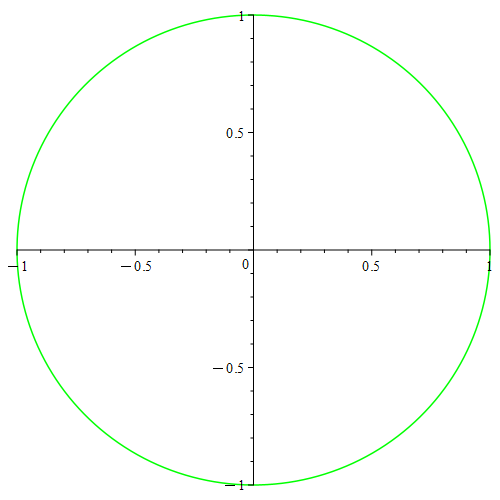
\includegraphics[scale=0.25]{Kurve_Plot cos(t), sin(t).png}
\caption{Plot von $c(t) = \left(\cos(t), \sin(t)\right)^\top$ für $t \in [0,2\pi]$}
\label{fig:Der Einheitskreis}
\end{Fig}

Das einfügen einer zwei im Sinus führt zu folgender Acht.
\begin{Fig}
\textbf{Die Acht}\\
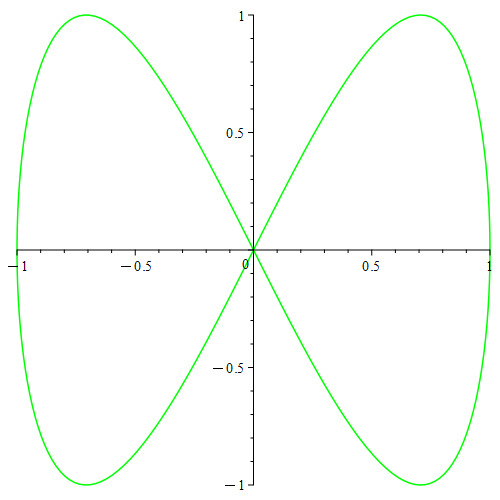
\includegraphics[scale=0.25]{Kurve_Plot cos(t), sin(2t).png}
\caption{Plot von $c(t) = \left(\cos(t), \sin(2t)\right)^\top$ für $t \in [0,2\pi]$}
\label{fig:Die Acht}
\end{Fig}

Weitere Beispiele und vor allem eigene Experimente lassen sich in \textit{1\_Kurve\_Plot.mw} machen. Sie haben ja bereits gesehen, was für einen großen Unterschied das Hinzufügen einer einfachen Zwei macht.

\subsection{Animation einer Kurve}
Jetzt möchte man natürlich nicht nur vor vollendete Tatsachen gestellt werden und ein langweiliges Bild anstarren\footnote{Tatsächlich hat es gerade beim Ausprobieren sehr viel Spaß gemacht auf eben diese Bilder zu starren.}. Deshalb haben wir eine Animation gebastelt.
\begin{Code}
Kurve\_Animation := proc(c, a, b)\\
local Kurve;\\
Kurve := proc(t) plot([[c(x)[1], c(x)[2], x = a .. t]], color = green); end proc;\\
animate([Kurve], [t], t = a .. b, frames = 50);\\
end proc:
\end{Code}
Es sei erwähnt, dass für diese Prozedur das Paket \texttt{plots} verwendet werden muss.\\
Innerhalb dieser Prozedur wurde noch eine Prozedur definiert. Die Prozedur \texttt{Kurve} gibt einfach für jedes $\mathtt{t}$ den Plot von $\mathtt{a}$ bis $\mathtt{t}$ aus. Für die Länge der Animation haben für 50 Frames gewählt\footnote{Alles andere hat sich zu schnell oder zu langsam angefühlt.}.\\
Ich würde Ihnen jetzt sehr gerne einige Animationen vorführen, aber das ist in \LaTeX{} leider nicht möglich\footnote{Ich habe tatsächlich eine Anleitung gefunden, aber diese ist viel zu kompliziert.}. Die folgende Sammlung von Bildern zeigt eine Animation von
\[c: [0, 2\pi] \rightarrow \mathbb{R}^2: t \mapsto \begin{pmatrix}
\cos(t^2) \\ t \sin(t)\end{pmatrix}\]
bei Frame 30, 40 und 50.
\begin{Fig}
\textbf{Das große Durcheinander}
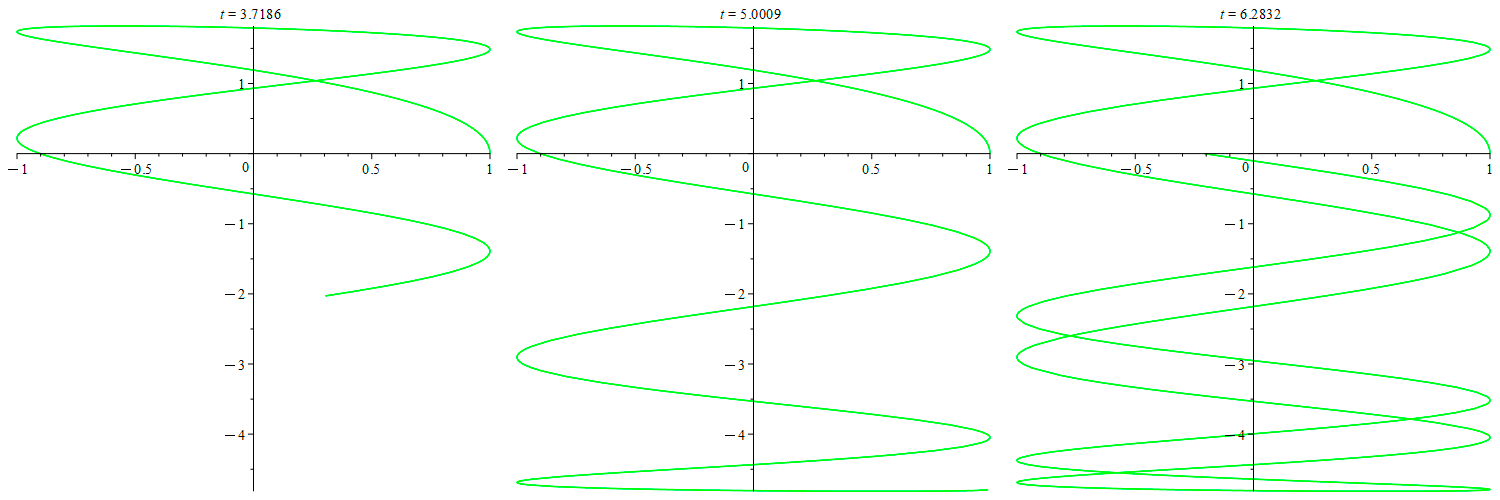
\includegraphics[scale=0.25]{Kurve_Animation cos(t^2), tsin(t).png}
\caption{\glqq Animation\grqq{} von $c(t) = \left(\cos(t^2), t\sin(t)\right)^\top$ für $t \in [0,2\pi]$}
\label{fig:Das große Durcheinander}
\end{Fig}

Einige weitere Animationen\footnote{Und diese sind tatächlich auch animiert.} lassen sich \textit{2\_Kurve\_Animation.mw} entnehmen.

\subsection{Länge einer Kurve}
Nun zu dem Thema, welches mir schon zuvor bekannt war. Die Länge einer Kurve bestimmen. Es gilt die folgende
\begin{Kasten}
\textbf{Definition:} Sei $c: [a,b] \rightarrow \mathbb{R}^2$ eine stetig differenzierbare Kurve. Die \textit{Länge} der Kurve von $a$ bis $b$ ist definiert als
\[L = \int_a^b \sqrt{x'(t)^2 + y'(t)^2} \d t~.\]
\end{Kasten}

\textbf{Bemerkung:}\\
Diese Formel sieht an sich sehr einfach aus. Doch hier sieht man deutlich das große Problem der Integralrechnung: Nicht jede integrierbare Funktion hat eine geschlossene Formel für die Stammfunktion. Dieses Problem wird uns auch später bei der Rekonstruktion einer Kurve aus ihrer Krümmung begegnen.\\
Man könnte sich natürlich auch fragen, ob der Integrand $\sqrt{x'(t)^2 + y'(t)^2}$ überhaupt integrierbar ist. Das ist tatsächlich eine gute Frage. Diese ist aber leicht zu beantworten, denn jede stetige Funktion ist auf einem kompakten Intervall integrierbar.\\
Nach Voraussetzung sind $x'(t)$ und $y'(t)$ stetig. Die Abbildungen $t \mapsto t^2$ und $t \mapsto \sqrt{t}$ sind ebenfalls stetig. Somit ist auch der Integrand als Linearkombination und Komposition stetiger Abbildungen wieder stetig, also integrierbar.\\

Nach dieser kurzen Einführung wollen wir mal eine solche Länge von Hand berechnen.\\
\textbf{Beispiel:}\\
Wir wollen nun der Einfachheit halber\footnote{Alles kompliziertere überlassen wir \textit{Maple}.} die Länge des Einheitskreises berechnen. Aus der Schule ist bekannt, dass für einen Kreis vom Radius $r > 0$ gelten sollte
\[L = 2 \pi r~.\]
Für den Einheitskreis muss also $L = 2 \pi$ sein. Wir wollen das nun nachrechnen. Betrachte dazu
\begin{align*}
L &= \int_0^{2\pi} \sqrt{(\cos(t)')^2 + (\sin(t)')^2} \d t\\
&= \int_0^{2\pi} \sqrt{(-\sin(t))^2 + (\cos(t))^2} \d t\\
&= \int_0^{2\pi} \sqrt{\sin^2(t) + \cos^2(t)} \d t~.\\
\intertext{Dank Additionstheorem ist $\sin^2(t) + \cos^2(t) = 1$ für alle $t \in [0, 2\pi]$. Somit gilt}
&= \int_0^{2\pi} \sqrt{1} \d t\\
&= \int_0^{2\pi} 1 \d t\\
&= \left[ t \right]_0^{2\pi} = 2\pi - 0 = 2 \pi~.\footnote{Hurra, wir haben richtig gerechnet. Interessant ist, dass \LaTeX{} diesen Teil zweimal als Fußnote ausgibt, obwohl ich ihn nur einmal eingetippt habe.}
\end{align*}
Es macht hier einen Unterschied, ob man den Einheitskreis über $[0,2\pi]$ oder über $[0,2n\pi]$ definiert. Es kommt entsprechend $L=2n\pi$ für den $n$-mal durchlaufenen Einheitskreis raus.\\
Dies war natürlich ein sehr einfaches Beispiel, aber gleichzeitig auch eines der einzigen, welches sich von Hand mit dem Hauptsatz der Differential- und Integralrechnung und (geschlossenen) Stammfunktionen lösen lässt.\\

Für genau diese komplizierten Fälle, in denen eine numerische Lösung nötig ist, haben wir die folgende Prozedur geschrieben.

\begin{Code}
Länge := proc(c, a, b)\\
local t, abl, l, L;\\
abl := map(diff, c(t), t);\\
L := evalf(int(norm(abl, 2), t = a .. b));\\
end proc:
\end{Code}

Dies ist tatsächlich nichts anderes als das, was wir vorher von Hand berechnet haben.\\

Für den Einheitskreis spuckt \textit{Maple} auch
\[L = 6.283185308 \approx 2 \pi\]
richtig aus.\\

Wir betrachten nun einen Teil der Neilschen Parabel gegeben durch
\[c: [-2,2] \rightarrow \mathbb{R}^2: t \mapsto \begin{pmatrix}
t^2 \\ t^3\end{pmatrix}~.\]

\begin{Fig}
\textbf{Die Neilsche Parabel}\\
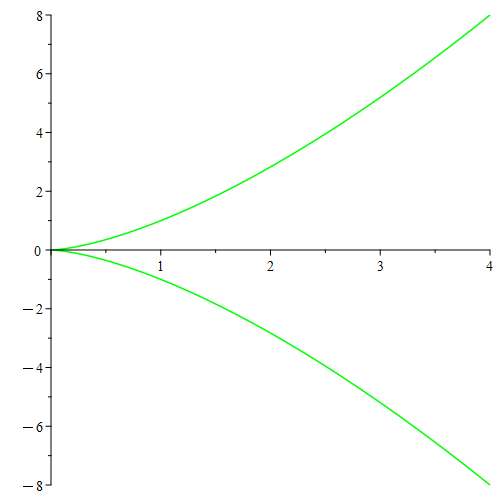
\includegraphics[scale=0.25]{Kurve_Plot t^2, t^3.png}
\caption{Plot von $c(t) = \left(t^2, t^3\right)^\top$ für $t \in [-2,2]$}
\label{fig:Die Neilsche Parabel}
\end{Fig}

Lässt man \textit{Maple} mit \texttt{Länge(c, -2, 2)} die Länge dieser Kurve berechnen, ergibt das
\[L \approx 18.14683058~.\]

Ein Problem tritt bei
\[c: [1,2] \rightarrow \mathbb{R}^2: t \mapsto \begin{pmatrix}
\tan(t)-1 \\ t(t^3-1)\end{pmatrix}\]
auf. Hier ist \textit{Maple} nicht in der Lage eine Länge zu Berechnen. Nach circa einer Minute an Rechenzeit gibt \textit{Maple} nur
\[L = \int_1^2 \left(\abs{1 + \tan^2(t)}^2 + 9 \abs{\operatorname{D}(t) (t^3-1)^2}^2 \abs{t}^4\right)^{\frac{1}{4}} \d t\]
aus. Trotz dem forcierten \texttt{evalf($\dots$)} wird hier kein Wert ausgerechnet\footnote{An dieser Stelle war ich etwas enttäuscht, weil bei all meinen Spielereien von Ableitungen über Integrale zu Differentialgleichungen, hat sich \textit{Maple} noch nie geweigert mir ein Ergebnis zu präsentieren.}.\\
Wir betrachten nun also den Plot von dieser scheinbar so schlimmen Kurve.
\begin{Fig}
\textbf{Die Kurve ohne Länge}\\
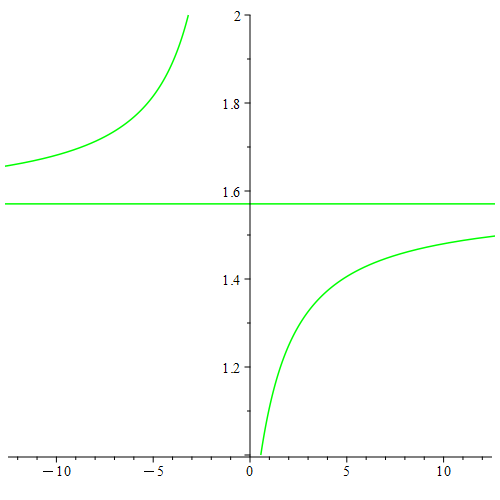
\includegraphics[scale=0.25]{Kurve_Plot tan(t) - 1, t(t^3 - 1).png}
\caption{Plot von $c(t) = \left(\tan(t)-1, t(t^3-1)\right)^\top$ für $t \in [1,2]$}
\label{fig:Die Kurve ohne Länge}
\end{Fig}

Mit bloßem Auge betrachtet sieht man, dass für die Länge $L$ gelten sollte\footnote{Gemessen in der Augenmetrik.}
\[45 \leq L \leq 50~.\]
Wenn man sich die Animation anschaut, sieht man, dass die $x$-Achsen parallele $y \approx 1.575$ extrem schnell durchlaufen wird. Ich vermute, dass sich die Berechnung des Integrals dort irgendwo aufhängt.\\

Bei der Berechnung weiterer Beispiele im \textit{Maple}-Skript fällt auf, dass hier teilweise etwas länger für die Werte der Integrale gerechnet wird. Es wird aber (fast) immer ein Ergebnis ausgespuckt.

\section{Kompliziertere Prozeduren}
Alles bisher präsentierte waren sehr einfache Prozeduren. Nun kommen wir zu etwas komplizierteren, die auch mal etwas an Überlegung benötigt haben.
\subsection{Tangente}
Die Tangente ist ein normierter Vektor, der die Richtung der Geschwindigkeit der Kurve darstellt.
\begin{Kasten}
\textbf{Definition:} Sei $c: [a,b] \rightarrow \mathbb{R}^2$ eine stetig differenzierbare Kurve. Die \textit{Tangente} in einem regulären Punkt $t \in [a,b]$ mit $c'(t) \neq 0$ ist definiert als
\[v(t) := \frac{c'(t)}{\dabs{c'(t)}}~.\]
\end{Kasten}

Wie immer betrachten wir den Einheitskreis.
\begin{Fig}
\textbf{Die Tangente an den Einheitskreis}\\
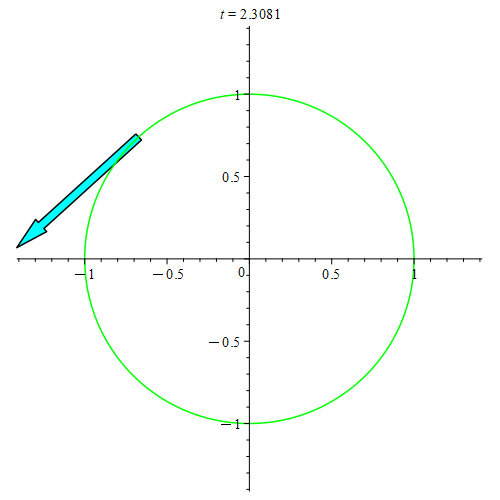
\includegraphics[scale=0.25]{Einheitskreis_Tangente.png}
\caption{Plot der Tangente bei $t \approx 2.31$ an $c(t) = \left(\cos(t), \sin(t)\right)^\top$}
\label{fig:Die Tangente an den Einheitskreis}
\end{Fig}

\subsection{Normale}
Die Normale ist ein normierter Vektor, der senkrecht zur Tangente steht.
\begin{Kasten}
\textbf{Definition:} Sei $c: [a,b] \rightarrow \mathbb{R}^2$ eine stetig differenzierbare Kurve. Die \textit{Normale} in einem regulären Punkt $t \in [a,b]$ mit $c'(t) \neq 0$ ist definiert als
\[v(t) := \frac{Jc'(t)}{\dabs{c'(t)}} \tab J = \begin{pmatrix}
0 & -1 \\ 1 & 0\end{pmatrix}~.\]
\end{Kasten}

Wie immer betrachten wir den Einheitskreis.
\begin{Fig}
\textbf{Die Normale an den Einheitskreis}\\
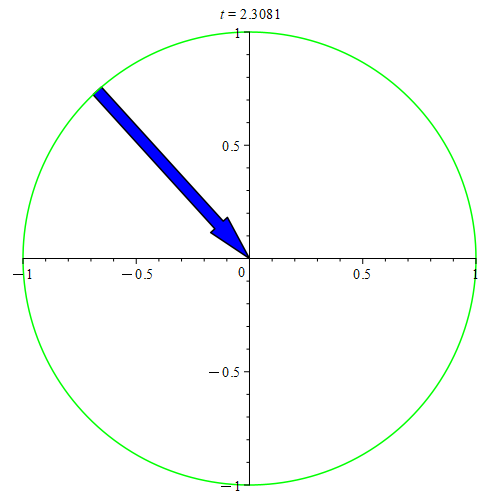
\includegraphics[scale=0.25]{Einheitskreis_Normale.png}
\caption{Plot der Normale bei $t \approx 2.31$ an $c(t) = \left(\cos(t), \sin(t)\right)^\top$}
\label{fig:Die Normale an den Einheitskreis}
\end{Fig}

\subsection{Animation zu Tangente und Normale}
Mit den Begriffen und Formeln zu Tangenten und Normalen bewaffnet, können wir uns nun einem der wichtigsten Teile dieses Berichtes widmen.\\
Wir haben eine Animation gemacht, wie sich die Tangente und Normale in Abhängigkeit von $t \in [a,b]$ auf der Kurve entlang bewegen. Die Prozedur ist gegeben durch\footnote{Lassen Sie die folgende Prozedur in ihrer vollen Schönheit auf sich wirken.}.

\begin{Code}
Tangente\_Normale\_Animation := proc(c, a, b)\\
local abl, J, n, n\_1, n\_2, v, v\_1, v\_2, Normale, Tangente, B;\\
abl := map(diff, c(t), t); J := <<0, 1> | <-1, 0>>;\\
n := MatrixVectorMultiply(J, abl)/norm(abl, 2);\\
n\_1 := unapply(n[1], t);\\
n\_2 := unapply(n[2], t);\\
v := abl/norm(abl, 2);\\
v\_1 := unapply(v[1], t);\\
v\_2 := unapply(v[2], t);\\
Normale := proc(t) plots[arrow]([c(t)], [n\_1(t), n\_2(t)], color = blue, symbolsize = 1, color = blue); end proc;\\
Tangente := proc(t) plots[arrow]([c(t)], [v\_1(t), v\_2(t)], color = green, symbolsize = 1, color = cyan); end proc;\\
B := plot([c(t)[1], c(t)[2], t = a .. b], color = green);\\
animate([Normale, Tangente], [t, t], t = a .. b, frames = 50, background = B, scaling = constrained);\\
end proc:
\end{Code}

Zuerst einmal ist es hier nötig neben \texttt{plots} auch \texttt{LinearAlgebra} zu verwenden, um die Matrix-Vektor-Multiplikation und die Normen verwenden zu können.\\
Auch in dieser Prozedur wurde nichts neues erfunden, sondern einfach die bisher definierten und gefundenen Dinge zusammengebaut.\\
Der Normalenvektor $\mathtt{n}$ wird wie in obiger Definition berechnet. Die Schwierigkeit bestand darin, dass \textit{Maple} zum einen die Matrix-Vektor-Multiplikation $\mathtt{J \cdot n(t)}$ nicht machen wollte und zum anderen auch nicht richtig normierte. Der so gewonnen Vektor wird anschließend in Partialfunktionen zerlegt, damit diese später animiert werden können.\\
Der Tangentenvektor $\mathtt{v}$ wird ähnlich berechnet und auch aufgeteilt.\\
Mit diesen Funktionen werden nun interne Prozeduren \texttt{Normale} und \texttt{Tangente} definiert, die zu jedem $\mathtt{t \in [a,b]}$ den Vektor berechnen, welcher von $\mathtt{c(t)}$ nach $\mathtt{v(t)}$ beziehungsweise $\mathtt{n(t)}$ zeigt.\\
$\mathtt{B}$ ist genau der Plot der Kurve, den wir aus dem ersten Teil kennen.\\
Zum Schluss werden diese Einzelteile durch \texttt{animate} in eine schöne Animation überführt.\\

Auch hier ist es wieder sehr Schade, dass ich Ihnen hier leider keine Animationen zeigen kann. Es sei auf \textit{4\_Tangente\_Normale\_Animation.mw} verwiesen.\\

Wir betrachten nun ein Kardioid\footnote{Oder auf deutsch \glqq Herzkurve\grqq{}, was ein sehr treffender Name ist, man rotiere einfach die folgende Abbildung um 90 Grad nach rechts.} gegeben durch
\[c: [0,2\pi] \rightarrow \mathbb{R}^2: t \mapsto \begin{pmatrix}
\cos^2(t) + \cos(t) \\ \sin(t) \cos(t) + \sin(t)\end{pmatrix}~.\]
In Frame 25, 26 und 40
\begin{Fig}
\textbf{Das Kardioid}\\
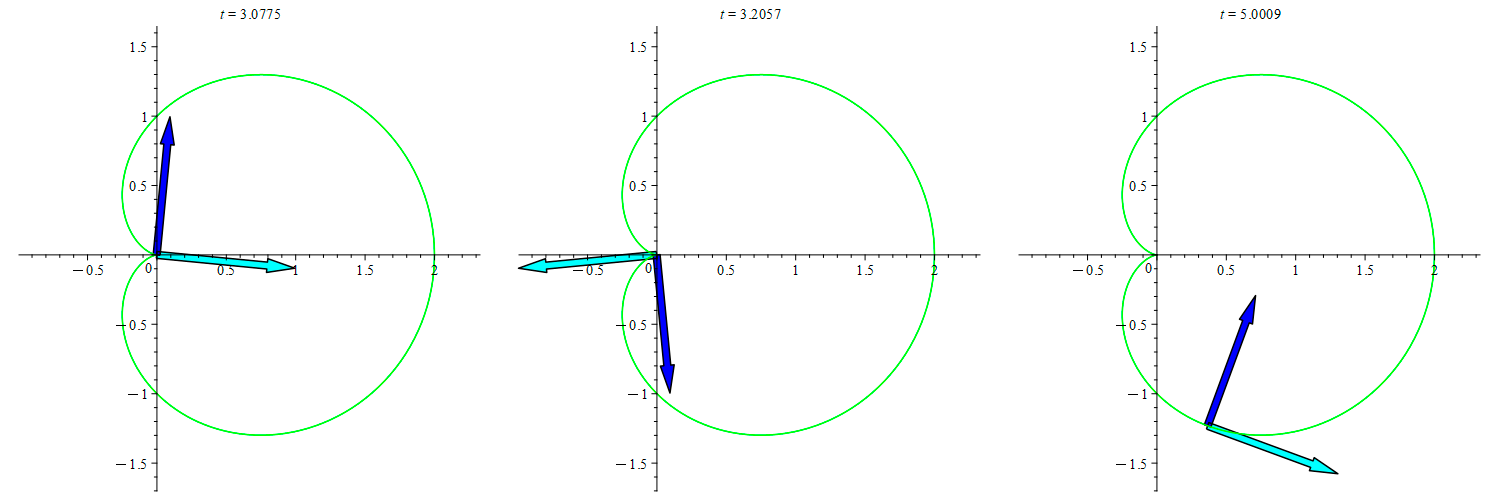
\includegraphics[scale=0.25]{T_N_Animaiton cos(t)^2 + cos(t), sin(t)cos(t) + sin(t).png}
\caption{\glqq Animation\grqq{} der Tangente und Normale von\\$c(t) = \left(\cos^2(t) + \cos(t), \sin(t) \cos(t) + \sin(t)\right)^\top$ für $t \in [0,2\pi]$}
\label{fig:Das Kardioid}
\end{Fig}
Hier fällt auf, dass \textit{Maple} die Vektoren an der bei $\pi$ überspringt. In diesem Punkt ist die Ableitung nicht regulär. Deshalb \glqq springen\grqq{} die Tangente und die Normale dort.

\section{Schwierige Prozeduren}
In diesem Teil werde ich einige Prozeduren vorstellen, welche von den Formeln aber vor allem auch durch ihre Implementierung sehr kompliziert waren.
\subsection{Krümmung einer Kurve}
\begin{Kasten}
\textbf{Definition:} Sei $c: [a,b] \rightarrow \mathbb{R}^2$ eine zweimal stetig differenzierbare Kurve. Die \textit{Krümmung} der Kurve in einem regulären Punkt ist definiert als
\[\kappa(t) := \frac{\det(c'(t), c''(t))}{\dabs{c'(t)}^3}~.\]
\end{Kasten}

\textbf{Bemerkung:}\\
Für eine nach Bogenlänge parametrisierte Kurve gilt
\[\kappa(t) = \skalar{c''(t), n(t)}~.\]
Da die obige Formel allgemeiner ist, haben wir nur diese implementiert.\\
Weiter ist eine Kurve \textit{rechtsgekrümmt}, falls $\kappa(t) < 0$ ist und \textit{linksgekrümmt}, falls $\kappa(t) > 0$. Die Art der Krümmung lässt sich den Animationen entnehmen. Positive Krümmungen liegen oberhalb der $x$-Achse und negative darunter.\\

Wie vorher wollen wir ein einfaches Beispiel von Hand berechnen.\\
\textbf{Beispiel:}\\
Es ist
\[c: [0, 2\pi] \rightarrow \mathbb{R}^2: t \mapsto \begin{pmatrix}
\cos(t) \\ \sin(t)\end{pmatrix}~.\]
Damit ist
\[c'(t) = \begin{pmatrix}
-\sin(t) \\ \cos(t)\end{pmatrix} \tab c''(t) = \begin{pmatrix}
-\cos(t) \\ -\sin(t)\end{pmatrix}~.\]
Es gilt
\[\det\begin{pmatrix}
-\sin(t) & -\cos(t)\\
\cos(t) & -\sin(t)
\end{pmatrix} = \sin^2(t) + \cos^2(t) = 1~.\]
Weiter ist
\[\dabs{c'(t)}^3 = \dabs{\begin{array}{c c} -\sin(t) \\ \cos(t) \end{array}}^3 = \sqrt {\sin^2(t) + \cos^2(t)}^3 = 1^3 = 1~.\]
Damit ist die Krümmung des Einheitskreises gegeben durch
\[\kappa(t) = 1~.\]
Der Einheitskreis ist also immer gleichstark linksgekrümmt.\\

In \textit{Maple} haben wir die folgende Prozedur programmiert
\begin{Code}
Krümmung\_einer\_Kurve := proc(c, a, b)\\
local abl, abl2, len, kappa, Kurve, Krümmung;\\
abl := map(diff, c(t), t);\\
abl2 := map(diff, abl, t);\\
len := sqrt(norm(abl, 2));\\
kappa := unapply(Determinant(<abl | abl2>)/len\^{}3, t);\\
Kurve := proc(t) plot([[c(x)[1], c(x)[2], x = a .. t]], color = green, scaling = constrained); end proc;\\
Krümmung := proc(t) plot([[x, kappa(x), x = a .. t]], color = yellow); end proc;\\
A := Array(1 .. 2);\\
A[1] := animate([Kurve], [t], t = a .. b, frames = 50);\\
A[2] := animate([`Krümmung`], [t], t = a .. b, frames = 50);\\
display(A);\\
end proc:
\end{Code}

Die Bestimmung von \texttt{kappa} läuft wie in obigem Beispiel. Wir haben uns dann dafür entschieden die Krümmungsfunktion und die Kurve in Abhängigkeit von $\mathtt{t}$ zu animieren. Deshalb wurden die zwei inneren Prozeduren \texttt{Kurve} und \texttt{Krümmung} verwendet, was je der Plot vom Zeitpunkt $\mathtt{a}$ bis zum Zeitpunkt $\mathtt{t}$ ist. Diese werden zum Schluss nebeneinander ausgegeben.\\

Die Neilsche Parabel liefert folgenden Plot.
\begin{Fig}
\textbf{Die geschweifte Klammer}\\
\includegraphics[scale=0.25]{Krümmung Neilsche Parabel.png}
\caption{Plot der Neilschen Parabel und ihrer Krümmung zu $t \in [-2,2]$.}
\label{fig:Die geschweifte Klammer}
\end{Fig}

Ein weiterer interessanter Plot ist.
\begin{Fig}
\textbf{Eine interessante Krümmung}\\
\includegraphics[scale=0.25]{Krümmung c_9.png}
\caption{Plot der Kurve und Krümmung zu \\$c(t) = (\cos(t) + \sin(t)^2, \sin(t) - \cos(t)^3)^\top$ für $t \in [0,2\pi]$.}
\label{fig:Eine interessante Krümmung}
\end{Fig}

Weitere Animationen befinden sich in \textit{5\_Krümmung\_einer\_Kurve.mw}
\subsection{Kurve aus Krümmung}
Nun stellt sich die Frage der Umkehrbarkeit dieser Operation. Die Antwort liefert der folgende
\begin{Kasten}
\textbf{Satz:} Sei $f: [a,b] \rightarrow \mathbb{R}$ eine beliebige glatte Funktion, dann existiert eine nach Bogenlänge parametrisierte Kurve $c : [a,b] \rightarrow \mathbb{R}^2$, die $f$ als Krümmung hat. Für die Partialfunktionen der Kurve gilt
\begin{align*}
\varphi(t) = \int_v^t f(u) \d u\\
x(t) = \int_v^t \cos(\varphi(u)) \d u\\
y(t) = \int_v^t \sin(\varphi(u)) \d u~.
\end{align*}
\end{Kasten}

\textbf{Bemerkung:}\\
Die untere Integrationsgrenze $v$ lässt sich beliebig verändern. Dies führt zu einer Verschiebung der Kurve.\\

Wie sonst auch wollen wir ein kleines Beispiel von Hand berechnen.\\
\textbf{Beispiel:}\\
Sei
\[f:[0,2\pi] \rightarrow \mathbb{R}: t \mapsto 1\]
eine Krümmungsfunktion. Es gilt
\begin{align*}
\varphi(t) &= \int_0^t f(u) \d u\\
&= \int_0^t 1 \d u\\
&= \left[ u \right]_0^t\\
&= t~.
\end{align*}
Damit ergibt sich
\begin{align*}
x(t) &= \int_0^t \cos(\varphi(u)) \d u\\
&= \int_0^t \cos(u) \d u\\
&= \left[ \sin(u) \right]_0^t\\
&= \sin(t)\\
y(t) &= \int_0^t \sin(\varphi(u)) \d u\\
&= \int_0^t \sin(u) \d u\\
&= \left[ -\cos(u) \right]_0^t\\
&= -\cos(t) + 1~.
\end{align*}
Somit ist die Kurve gegeben durch
\[c: [0,2\pi] \rightarrow \mathbb{R}^2: t \mapsto \begin{pmatrix}
\sin(t) \\ -\cos(t) -1\end{pmatrix}~.\]
Das geübte Auge erkennt hierin den verschobenen Einheitskreis. Dies stimmt also mit dem Ergebnis aus dem vorherigen Kapitel überein.\\

Die \textit{Maple}-Prozedur lautet.
\begin{Code}
Kurve\_aus\_Krümmung := proc(f, a, b)\\
local t, u, phi, x, y, c, Kurve, Krümmung;\\
phi := int(f(u), u = 0 .. t);\\
x := int(cos(phi), t = 0 .. s);\\
y := int(sin(phi), t = 0 .. s);\\
Kurve := proc(t) plot([[x, y, s = a .. t]], color = green); end proc;\\
animate([Kurve], [t], t = a .. b, frames = 50);\\
end proc:
\end{Code}

Wie immer ist dies einfach die Ausführung der Rechnung aus obigem Beispiel.\\
Die riesige Schwierigkeit war es hinzubekommen, dass \textit{Maple} hier richtig rechnet. Aus diesem Grund wechseln sich in der Prozedur auch die Integrationsvariablen. Außerdem war es hier wichtig nicht die Funktion $\mathtt{phi(t)}$ zu integrieren, sondern den Ausdruck $\mathtt{phi}$.\\
Ansonsten haben wir uns hier auch wieder für die bereits bekannte Animation entschieden, denn gerade das folgende Beispiel sieht damit viel besser aus.\\
Betrachte die Kurve
\[c: [2-\pi,2\pi] \rightarrow \mathbb{R}: t \mapsto t~.\]

\begin{Fig}
\textbf{Die Doppel-Schleife}\\
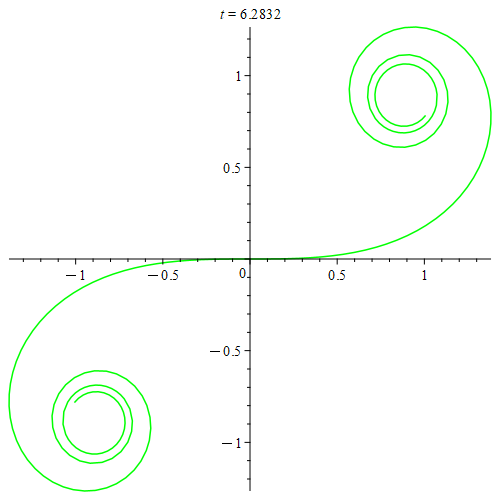
\includegraphics[scale=0.25]{Kurve zu t.png}
\caption{Plot zur Kurve aus der Krümmung $f(t) = t$ für $t \in [-2\pi,2\pi]$.}
\label{fig:Die Doppel-Schleife}
\end{Fig}
Es fällt auf, dass die meisten Kurven aus einer Krümmung irgendwelche Schleifen, machen, welche scheinbar auf einen Punkt konvergieren.\\
Weitere Beispiele dazu befinden sich in \textit{6\_Kurve\_aus\_Krümmung.mw}. Als letztes Beispiel sei
\[f: [-4\pi,4\pi] \rightarrow \mathbb{R}: t \mapsto \sin(t)~.\]
\begin{Fig}
\textbf{Die Schlange}\\
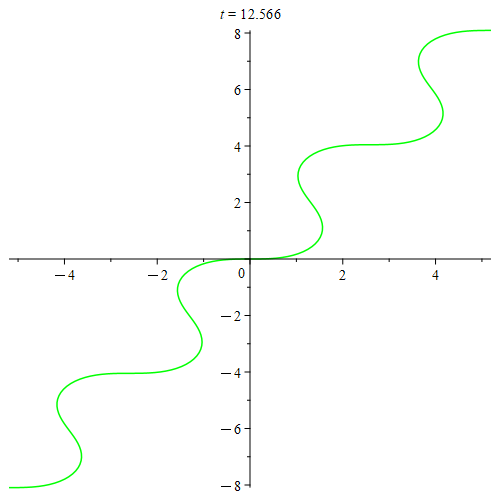
\includegraphics[scale=0.25]{Schalge f_7.png}
\caption{Plot der Kurve aus der Krümmung $f(t) = \sin(t)$ für \\$t \in [-4\pi,4\pi]$.}
\label{fig:Die Schlange}
\end{Fig}
Dies ist zwar kein Strudel, aber trotzdem ein interessanter Plot.\\

Mit diesem Plot möchte ich meinen Bericht beenden. Wir haben noch Programme geschrieben, welche sich mit Evolute und Evolvente beschäftigen. Diese liegen als siebtes und achtes Skript bei\footnote{Sie heißen \textit{7\_Evolute.mw} und \textit{8\_Evolvente.mw}}. Hier lassen sich auch einige schöne Plots betrachten, aber diese würden diesen nun schon 24 Seiten langen Bericht in meinen Augen sprengen. Es lohnt sich generell einen Blick in die Skripte zu werfen, da sich dort eine sehr große Anzahl an Beispielen befindet, welche diesen Bericht durch die Vielzahl an Bildern nur in die Länge gezogen hätten.\\

Das arbeiten mit \textit{Maple} und \LaTeX{} hat sehr viel Spaß gemacht\footnote{Das Wort \textit{Maple} kommt nun insgesamt 33 mal in diesem Text vor.}.

\newpage

\section{Abbildungen}
In diesem Teil sind die Kurven und Funktionen zu den jeweils verwendeten Abbildungen. Es ist absolut unnötig diesen Teil zu \glqq lesen\grqq{} er ist nur zur Vollständigkeit da, um nachvollziehen zu können, woher die Bilder kommen.
\begin{scriptsize}
Abbildung \ref{fig:Der Einheitskreis}:\\
\texttt{c\_1 := t -> <cos(t), sin(t)>}\\
\texttt{Kurve\_Plot(c\_1, 0, 2*Pi)}\\

Abbildung \ref{fig:Die Acht}:\\
\texttt{c\_2 := t -> <cos(t), sin(2*t)>}\\
\texttt{Kurve\_Plot(c\_2, 0, 2*Pi)}\\

Abbildung \ref{fig:Das große Durcheinander}:\\
\texttt{c\_5 := t -> <cos(t\^{}2), t*sin(t)>}\\
\texttt{Kurve\_Animation(c\_5, 0, 2*Pi)}\\

Abbildung \ref{fig:Die Neilsche Parabel}:\\
\texttt{c\_6 := t -> <t\^{}2, t\^{}3>}\\
\texttt{Kurve\_Plot(c\_6, -2, 2)}\\

Abbildung \ref{fig:Die Kurve ohne Länge}:\\
\texttt{c\_7 := t -> <tan(t) - 1, t(t\^{}3 - 1)>}\\
\texttt{Kurve\_Plot(c\_7, 1, 2)}\\

Abbildung \ref{fig:Die Tangente an den Einheitskreis}:\\
\texttt{c\_1 := t -> <cos(t), sin(t)>}\\
\texttt{Tangente\_Normale\_Animation(c\_1, 0, 2*Pi)}\\
Modifiziert durch entfernen von allem, was mit \texttt{Normale} zusammenhängt.\\

Abbildung \ref{fig:Die Normale an den Einheitskreis}:\\
\texttt{c\_1 := t -> <cos(t), sin(t)>}\\
\texttt{Tangente\_Normale\_Animation(c\_1, 0, 2*Pi)}\\
Modifiziert durch entfernen von allem, was mit \texttt{Tangente} zusammenhängt.\\

Abbildung \ref{fig:Das Kardioid}:\\
\texttt{c\_8 := t -> <cos(t)\^{}2 + cos(t), sin(t)*cos(t) + sin(t)>}\\
\texttt{Tangente\_Normale\_Animation(c\_8, 0, 2*Pi)}\\

Abbildung \ref{fig:Die geschweifte Klammer}:\\
\texttt{c\_6 := t -> <t\^{}2, t\^{}3>}\\
\texttt{Krümmung\_einer\_Kurve(c\_6, -2, 2)}\\

Abbildung \ref{fig:Eine interessante Krümmung}:\\
\texttt{c\_9 := t -> <cos(t) + sin(t)\^{}2, sin(t) - cos(t)\^{}3>}\\
\texttt{Krümmung\_einer\_Kurve(c\_9, 0, 2*Pi)}\\

Abbildung \ref{fig:Die Doppel-Schleife}:\\
\texttt{f\_2 := x -> x}\\
\texttt{Kurve\_aus\_Krümmung(f\_2, -2*Pi, 2*Pi)}\\

Abbildung \ref{fig:Die Schlange}:\\
\texttt{f\_7 := x -> sin(x)}\\
\texttt{Kurve\_aus\_Krümmung(f\_7, -4*Pi, 4*Pi)}
\end{scriptsize}

\newpage

\section{Fußnoten}
\theendnotes
\end{document}
